% Header
\renewcommand\evenpagerightmark{{\scshape\small Chapter 7}}
\renewcommand\oddpageleftmark{{\scshape\small Summary and outlooks}}

\hyphenation{}

\chapter[Summary and outlooks]{Summary and outlooks}
\label{chapt7}

	\section{Summary}
	\label{chapt7:sec:summary}
	
	The upgrade of the \acf{LHC} toward the \acf{HL-LHC} started in 2018. It aims at increasing the luminosity of the accelerator to boost its discovery potential. Many extensions to the \acf{SM} feature \acf{HSCPs} which, in the context of the \acf{CMS}, could be identified thanks to its muon system. An increase in instantaneous luminosity will mechanically result into an increase of the background noise and of the irradiation levels the machines will be subjected to. The current muon system needs to be certified for the HL-LHC period. On the other hand, additional Resistive Plate Chambers (RPCs) will be installed in the region closest to the beam line. The goal is to ensure the best quality possible of the muon trigger by mitigating the background effects and increasing the redundancy of the trigger system. The CMS RPC upgrade has been and will keep on being an exciting scientific research. The collaboration converged towards the solutions that will be adopted in the perspective of HL-LHC. Even though the consolidation of the present CMS RPC infrastructure and the certification of the new technologies that will complete the redundancy of the muon system are still ongoing, the future of the experiment from the RPC point of view is now clear. To reach this point, my contribution during the preliminary phase of tests between 2012 and 2015 has been decisive in both the consolidation of the present detectors and in the selection of the \acl{FEE} that will equip the improved RPCs (iRPCs). At every step, I played an important role in setting up the experiments but also in gathering and analysing the data.
	
	My first contribution to the CMS Upgrade was the testing of two selected potential FEE technologies: a low-noise preamplifier using SiGe technology and developed at INFN Tor Vergata, and FEEs based on the PETIROC ASIC also featuring SiGe technology and used for \acl{ToF} applications. At two occasions, the INFN preamplifier has been tested and compared to the current CMS FEEs. In a first experiment, the preamplifier was directly connected to four read-out strips and the output signal was digitized by the use of a discriminator. The preamplifier was operated with a charge threshold as low as \SI{3}{fC} and showed a working voltage shift of \SI{475}{V} with respect to the RPC operated with the current CMS electronics. To improve the comparison of the INFN technology with the CMS FEB, a FEB without preamplifer was designed to connect and operate the preamplifier. This way, the comparison would directly concern the low-noise candidate to the current preamplification stage used by CMS. The electronics were mounted on spare CMS RPCs to repeat the previous experiment. The shift in working voltage observed reached \SI{410}{V} at a threshold of \SI{5}{fC}, consistent with the first result obtained.\\
	The FEEs developed by OMEGA were tested on a spare CMS RPC gap from the RE4 production. For comparison purposes, the spare gap used was mounted into a RPC case and the detector was operated in single gap mode with the CMS FEB. The results showed that the HARDROC2 could provide a reduction of the working voltage in single gap mode of almost \SI{500}{V} at charge sensitivity of \SI{121.4}{fC}, comparable to the threshold of the CMS FEEs set at \SI{146}{fC}, while keeping noise levels below \SIrate{0.1}. Moreover, this technology had already been certified through multiple experiments using detectors such as scintillators and RPCs. Finally, it had the advantage of proposing a 2D read-out that would greatly improve the spatial resolution of the detectors in the radial direction. The expertise of the Intrumentation group was demonstrated in this campaign.\\
	The certification of the resulting technologies, adapted for the needs of CMS in the RE3/1 and RE4/1 regions of the muon endcaps, is being performed at the \acf{GIF++} where an irradiation bunker along a muon beam had been built. The facility featured a \SI{14}{TBq} Cesium source. The pupose of this new facility was to conduct various long term studies in the perspective of the HL-LHC. The prototypes for the improved CMS chambers are trapezoidal double-gap RPCs featuring \acf{HPL} electrodes of \SI{1.4}{mm} and gas gaps of the same thickness. The reduction of the gap thickness was motivated by the lower gain of such detectors at similar electric field. The read-out PCB consists in 96 longitudinal strips with a pitch ranging from \SI{4}{mm} at the narrow end to \SI{8}{mm} at the wide end. This design defines the baseline of what will be installed in CMS in the future. Several prototypes have been assembled and are used to test the CMS RPCROC FEEs derived from the PETIROC technology and the INFN Tor Vergata alternative that was adapted to the requirements of the CMS RPC.\\
	For comparison purposes, cosmic tests without irradiation have first been conducted on the iRPC prototypes using the current CMS FEBs. The detector reaches its working voltage at \SIerror{7383}{70}{V} with an efficiency near 97\% when operated at a threshold of \SI{133}{fC}. The mean muon cluster size is measured to be \numerror{2.4}{0.1} strips and the noise rate is of the order of \Ord{-1}\,\sirate.\\
	Two versions (FEBv0 and FEBv1) of CMS RPCROC based on the PETIROC ASIC coupled to an FPGA have been tested so far and FEBv2 is in preparation. The CMS RPCROC is designed to read-out the 96 pick-up strips from both ends, providing a 2D information about the location of the received hits. FEBv0 was operated at a threshold of \SI{100}{fC} while FEBv1 was operated at a lower threshold of \SI{50}{fC} thanks to a PETIROC with reduced cross-talk. Without irradiation, the prototype equipped with FEBv1 reached 99\% of efficiency at a working voltage of \SI{7250}{V}. At a background hit rate of \SIkrate{2}, the working voltage shifted to \SI{7340}{V} with an efficiency of 95\%. However, the Cyclone V FPGA and PETIROC2B ASIC suffered from radiation hardness issues. The new FEBv2 will feature a new version of the Cyclone V FPGA especially developed to address applications in irradiated environments. The new PETIROC2B is being tested at the LLN neutron beam up to a fluence of \Ord{14}\,\si{pC/cm^2} which should be five times more than what is expected at CMS.\\
	The INFN FEEs feature eight preampliers of the same type than what had been tested in the preliminary tests as well as two discriminator ASICs. Hence, twelve of these FEEs were integrated and soldered on the read-out PCB whose pick-up strip are terminated with \SI{50}{\Ohm} resistors. The detector was operated with a threshold of \SI{5}{fC} and was irradiated up to a background hit rate about \SIrate{4} at which it kept an efficiency above 92\%. Without irradiation, the prototype has an efficiency greater than 99\% at a working voltage below \SI{7000}{V}. The mean muon cluster size is measured to be \numerror{3.4}{0.1}, larger than in the case of the CMS FEB due to the higher sensitivity. At a rate of \SIrate{2}, the efficiency was near 97\% at a working voltage of \SI{7250}{V}. Due to the irradiation, the mean muon cluster size dropped to \numerror{2.6}{0.1}.
	
	Nonetheless, my greatest contribution to the upgrade took place at the level of the longevity and certification study of the present CMS RPC system. I joined the preliminary study that first took place at the old \acl{GIF} of CERN in which a Cesium source with an activity of \SI{494}{GBq} was available. A first setup with a single spare CMS RPC was the occasion to develop the first hints of \acl{DAQ}, \acl{DQM} and data analysis tools. The chamber was installed in the bunker in front of the radioactive source to be irradiated at a background hit rate of \SIrate{600}. The performance of the detector was probed using a cosmic muon telescope serving as trigger. The results suggested that the performance of the detector had dropped to 80\% of efficiency with a working voltage shifted to higher values by \SI{1000}{V} at \SIrate{600}.\\
	A larger scale experiment was then designed at the GIF++. The new setup consists of two spare RE2/2 CMS RPCs built in 2007 and oof two spare RE4/2 built in 2013. One chamber of each type serves as reference while the second is used for longevity studies under irradiation. According to extrapolations CMS data, the detectors of the present system would need to be certified for a background rate of \SIrate{600} and without significative loss of performance at a total integrated charge of \SI{840}{mC/cm^2}, corresponding to three times the worst background hit rate extrapolated from CMS data in a RPC.\\
	Respectively 74 and 40\% of the planned integrated charge program have been performed since 2016. The monitoring of the current density and of the background hit rate show a strong correlation with the temperature at the GIF++. When taken into account, the current density and background rate monitored in the irradiated detectors show a decrease relative to the reference detectors. This effect seems to be correlated with an increase in resistivity of the irradiated detectors of a factor 2 relative to the reference RPCs. However, the fluctations of the current density and background hit rate ratios show a correlation with the relative humidity of the gas mixture. The effect seems then reversible by operating the chambers at a higher relative humidity level.\\
	No loss in performance was observed at a background rate of \SIrate{600}. All the detectors show an efficiency beyound 94\% up to the required background level. The recorded shift in working voltage of \SI{100}{V} for the RE2 RPCs and of 300 to \SI{500}{V} for the RE4 RPCs is consistent with the difference in electrode resistivities of both detector types. The RE2 detectors have a resistivity in the range between 1 and \Sci{3}{10}\,\si{\ohm\cdot cm} while the newer RE4 have a resistivity between 0.7 and \Sci{2}{11}\,\si{\ohm\cdot cm}. The gamma irradiation generates a voltage drop over the electrodes proportionnal to their resistance. As the electrodes behave as capacitors, this voltage drop that is usually negligible without irradiation decreases the effective electric field in the gas volume at a given applied voltage when the rate of incoming gamma particles increases. When taken into account, the working voltage shift disappears. The remaining monitored parameters such as the efficiency, the mean muon cluster size, or the charge deposition per avalanche, do not show any difference between the reference and irradiated detectors.\\
	At this stage, the CMS RPC group is on the way of certifying the current RPC system for the HL-LHC period. The longevity study should be completed by the end of 2021. With the upgrade of the Link-system, the present detectors should live through the high-luminosity phase of the LHC without important change in their performance.

	\section{Outlooks}
	\label{chapt7:sec:outlooks}
	
	\paragraph*{About the longevity studies at the GIF++:} In order to improve the quality of the certification tests performed at the GIF++, several points could be studied. First of all, the temperature correction used, although the same than the one used at CMS, is not efficient enough to prevent strong fluctuations of the current density and of the background hit rate measured by the detectors. The use of \acl{PCA} helped in understanding the reasons for the fluctuations. To ensure the good quality of the study and make sure that even small effects could be monitored, a better control of the temperature in the bunker, or at least around the detectors, could be achieved. In the case where it would be too complex to stabilize the temperature of such a large area, more care should be put into the study of the temperature effects on the detectors installed at the GIF++.\\
	The fluctuations of the irradiated-over-reference ratio of current density and background hit rate probably find there origin in a fluctuation of the resistivity. This fluctuation was showed to be correlated to the fluctuation of gas relative humidity, it is important to seek and repair any potential gas leak at the level of the detectors and to change the algorithm used to stabilize the humidity inside of the detectors. The humidity of the gas mixture in the supply line is now kept very stable by constantly monitoring its value and adjusting the flows of humidified and dry gas lines. It is suggested to try keeping stable the relative humidity of the gas on the exhaust line instead. The humidity of the supply should vary to correct for the loss of humidity along the setup and a stable exhaust humidity would ensure stable working conditions for the detectors.
	
	\paragraph*{About the search for eco-friendly gas mixtures:} The present thesis document unfortunately only focusses on the R\&D produced by the CMS RPC team on the present and new detection technologies that are and will be used at CMS. Few information about the very important research being conducted in order to find a replacement to the standard RPC gas mixture is provided. The outcome of this search for new gases will be of major interest as the restriction for the standard mixture will get harder.
	
	\paragraph*{About the future of the Instrumentation Group at the University of Ghent:} Once the R\&D is complete, the next phase will consist in the upgrade of the RPC sub-system. The Instrumentation Group will mainly take part in quality control of the assembled detectors for the expension of the endcaps as was already the case for the production of the RE4 detectors for the fourth endcap disk of CMS between 2012 and 2013. This phase should start during the second half of 2020, as can be seen in Figure~\ref{fig:milestones}. In this perspective, the instrumentation laboratory is being prepared and will be the training site for the technicians and physicists of the institutes where the detectors will be assembled. Improved RPC demonstrators will be installed in CMS during the \acl{YETS} of winter 2021/2022 and the installation of the remaining detectors should take place in January 2023. After LS3, the LHC will finally enter its high-luminosity phase and new breakthrough will be foreseen. The good performance of the RPCs and of all of CMS sub-systems will be important in this reguard and the skills developed during the present R\&D will become an important asset in maintaining the performance of the detectors at their best level.
	
	\begin{figure}[H]
	    \centering
	    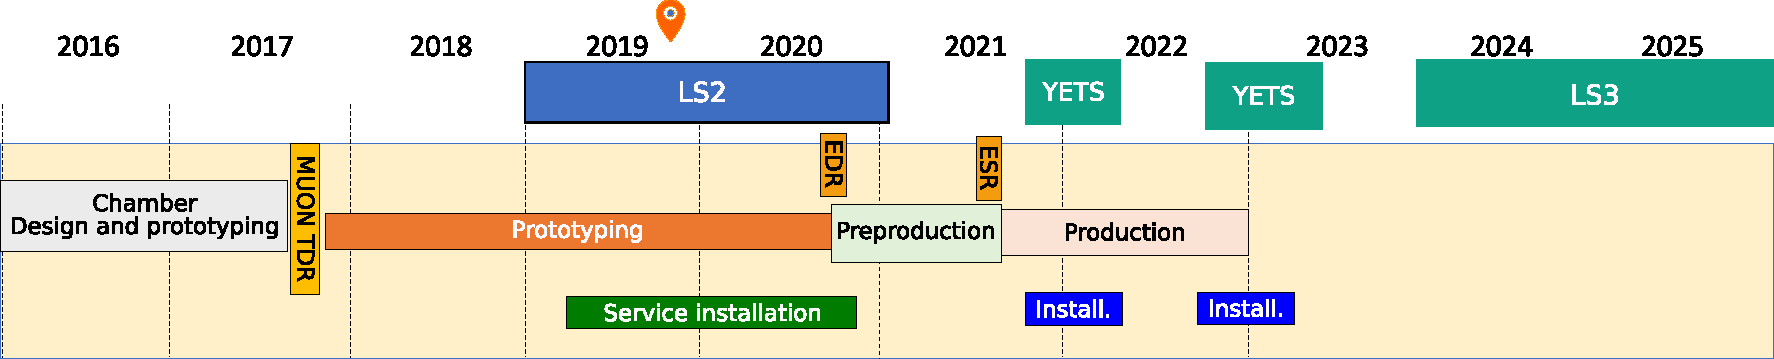
\includegraphics[width=\linewidth]{fig/chapt7/CMS-RPC-Milestones.pdf}
	    \caption{\label{fig:milestones} RE3/1 and RE4/1 prototyping and production schedule.}
	\end{figure}

\clearpage{\pagestyle{empty}\cleardoublepage}